\documentclass[12pt, a4paper]{report}
\usepackage[utf8]{inputenc}
\usepackage{graphicx}
\usepackage{nameref}
\graphicspath{ {Pictures/} }
\usepackage{hyperref}
\hypersetup{
    colorlinks=true,
    linkcolor=blue,
    filecolor=magenta,      
    urlcolor=red,
}
\usepackage{geometry}
\usepackage{float}
\usepackage{algorithm}
\usepackage{algpseudocode}
\usepackage{amsmath, bm}
\usepackage[export]{adjustbox}
\usepackage{subcaption}
\usepackage{mathabx}
 

\title{%  
Homework Assignment 3 
   \\
  \large  Dynamics Of Non Linear Robotic Systems}
\author{Ilia Sevostianov %\thanks{thanks to God}
    }
\date{\today}

\begin{document}
	\maketitle

\begin{figure}[H]
	\centering
		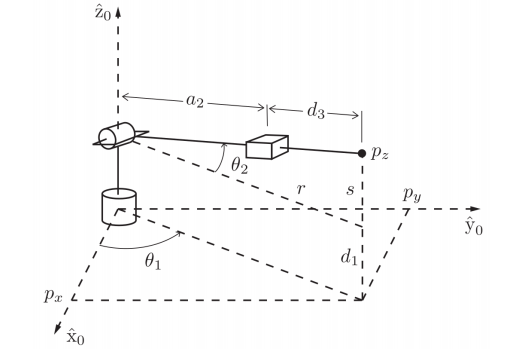
\includegraphics[width=0.6\textwidth]{Image1} % File
	\caption{RRP robot.} % Name
	\label{fig:mesh1}
\end{figure}

\section*{Task 1:}
Derive FK equations for the robot depicted in figure \ref{fig:mesh1}. Use $\theta_1$, $\theta_2$, $d_3$ as
joint space variables, $p_x$, $p_y$, $p_z$ as operational space variables. Parameters
$d_1$, $a_2$ are known (assign them some positive values for succeeding tasks).

{\centering
\subsection*{Solution}
}

\begin{figure}[H]
	\centering
		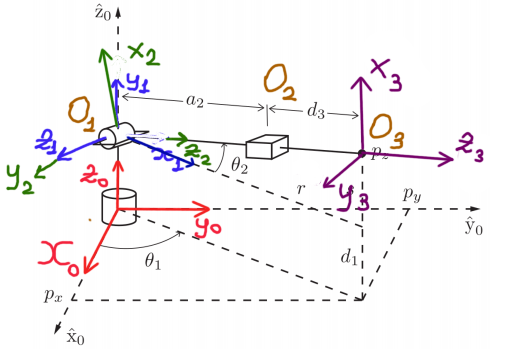
\includegraphics[width=0.6\textwidth]{Image2} % File
	\caption{RRP robot: joint axes} % Name
	\label{fig:mesh2}
\end{figure}

Let's derive FK equations for the robot: 


\begin{equation}
        \bm{O_1} =
        \begin{bmatrix}
                0\\
                0\\
                d_1
        \end{bmatrix}
\end{equation}

\begin{equation}
        \bm{O_2} =
        \begin{bmatrix}
                a_2c_2c_1\\
               a_2c_2s_1\\
                d_1+a_2s_2
        \end{bmatrix}
\end{equation}

\begin{equation}
        \bm{O_3} =
                \begin{bmatrix}
                p_x\\
               p_y\\
                p_z
        \end{bmatrix}
        =
        \begin{bmatrix}
                a_2c_2c_1+d_3c_2c_1\\
               a_2c_2s_1+d_3c_2s_1\\
                d_1+a_2s_2+d_3s_2
        \end{bmatrix} 
        = 
        \begin{bmatrix}
                c_2c_1(a_2+d_3)\\
               c_2s_1(a_2+d_3)\\
                d_1+s_2(a_2+d_3)
        \end{bmatrix}
\end{equation}

\section*{Task 2} \label{sec:Task 2}
 Derive IK equations.

{\centering
\subsection*{Solution}
}

In IK we assume that we know coordinates of the tool:

\begin{equation}
        \bm{p} =
        \begin{bmatrix}
                p_x\\
               p_y\\
                p_z
        \end{bmatrix}
\end{equation}

Let's start from angle $\theta_1$ (see figure \ref{fig:mesh2}):

\begin{equation}
        \theta_1 = atan2(p_y, p_x)
\end{equation}

\begin{equation}
        s = p_z - d_1, 
        r = \sqrt{p_x^2+p_y^2}
\end{equation}

So, we can calculate $\theta_2$:

\begin{equation}
        \theta_2 = \frac{\pi}{2}+atan2(s, r)
\end{equation}

To calculate $d_3$ we must write the next equation for the triangle:

\begin{equation}
        r^2 +s^2 = {(a_2+d_3)}^2
\end{equation}

\begin{equation}
        r^2 +s^2 = a_2^2+2a_2d_3+d_3^2
\end{equation}


\begin{equation}
        d_3^2+2a_2d_3+a_2^2 -r^2-s^2 = 0 
\end{equation}

Let's find $d_3$:

\begin{equation}
        D = 4(a_2^2-a_2^2+r^2+s^2) = 4(r^2+s^2)
\end{equation}

\begin{equation}
	        d_3 = {{-2a_2 \pm \sqrt{D}}\over{2}} = {{-2a_2 \pm 2\sqrt{r^2+s^2}}\over{2}} = -a_2 \pm \sqrt{r^2+s^2}
\end{equation}

We exclude negative solution because it's impossible for out robot's configuration. So, 

\begin{equation}
	        d_3 = -a_2 + \sqrt{r^2+s^2}
\end{equation}

Also, here is the second valid solution for $\theta_1$ and $\theta_2$:

\begin{equation}
        \theta_1 = \pi + atan2(p_y, p_x)
\end{equation}

\begin{equation}
        \theta_2 = \frac{3\pi}{2}- atan2(s, r)
\end{equation}

To conclude: 

\begin{equation}
        \bm{q} =
        \begin{bmatrix}
                \theta_1\\
               \theta_2+\frac{\pi}{2}\\
                d_3
        \end{bmatrix}
        = 
        \begin{bmatrix}
                atan2(p_y, p_x)\\
               \frac{\pi}{2}+atan2(s, r)\\
                -a_2 + \sqrt{r^2+s^2}
        \end{bmatrix}       
\end{equation}

And the second solution:

\begin{equation}
        \bm{q} =
        \begin{bmatrix}
                \theta_1\\
               \theta_2+\frac{\pi}{2}\\
                d_3
        \end{bmatrix}
        = 
        \begin{bmatrix}
                \pi + atan2(p_y, p_x)\\
              \frac{3\pi}{2} - atan2(s, r)\\
                -a_2 + \sqrt{r^2+s^2}
        \end{bmatrix}       
\end{equation}
\section*{Task 3:}
Compute the manipulator Jacobian for representation of linear and angular velocity of point \textbf{p}.
\begin{itemize}
	\item Use classical approach (partial derivatives).
\item Use geometric approach (cross products).
\end{itemize}


{\centering
\subsection*{Solution}
}

Jacobian is the matrix that relates the linear and angular velocity of the end-effector to the vector of joint velocities \textbf{$\dot{q}(t)$}:

\begin{equation}
        \begin{bmatrix}
                \dot{x}\\
                \dot{y}\\
                \dot{y} \\
                {w_x} \\
                {w_y} \\
                {w_z} \\
        \end{bmatrix}= \bm{J}\bm{\dot{q}}   
        \label{eq:18}
\end{equation}

where J is Jacobian.

{\centering
\subsubsection*{Classical Approach}
}

In this approach the formula in figure \ref{fig:mesh3} is used.
\begin{figure}[H]
	\centering
		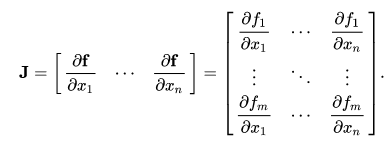
\includegraphics[width=0.6\textwidth]{Image3} % File
	\caption{Formula for the Jacobian calculation } % Name
	\label{fig:mesh3}
\end{figure}

So, I made the matlab script to calculate the Jacobian of my sistem. The idea is that we obtained the coordinate $O_i$ in FK. And to calculate Jacobian we must calculate partial derivatives of this matrixes by \textbf{q}. 

Let me show the part of the matlab code, that calculates Jacobian, in figure \ref{fig:mesh4}(I assumed \textbf{q} as [theta1 theta2 d3]):


\begin{figure}[H]
	\centering
		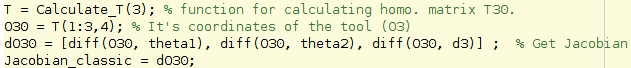
\includegraphics[width=0.8\textwidth]{Image4} % File
	\caption{MATLAB code to calculate Jacobian} % Name
	\label{fig:mesh4}
\end{figure}

After implementation this, I obtained the result shown in figure \ref{fig:mesh5}.

\begin{figure}[H]
	\centering
		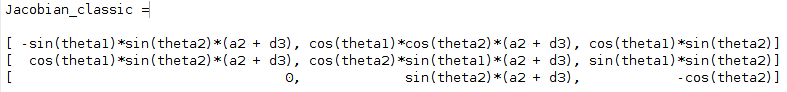
\includegraphics[width=1.0\textwidth]{Image5} % File
	\caption{Jacobian by Classical Approach} % Name
	\label{fig:mesh5}
\end{figure}


{\centering
\subsubsection*{Geometrical Approach}
}

In this approach the formulas in the table \ref{table:1} is used.

\begin{table}[H]
\centering
\begin{tabular}{ |c||c||c|}
 \hline
 \multicolumn{3}{|c|}{Formulas for Jacobian's parts calculation} \\
 \hline
  & Prismatic & Revolute \\
 \hline
 Linear & $
        J_v ={R_{i-1}}^0
        \begin{bmatrix}
                0\\
               0\\
                1
        \end{bmatrix}$ 
& $
        J_v ={R_{i-1}}^0
        \begin{bmatrix}
                0\\
               0\\
                1
        \end{bmatrix}({d_{n}}^0-{d_{i-1}}^0)$ \\
 Rotational & $
        J_w =
        \begin{bmatrix}
                0\\
               0\\
                0
        \end{bmatrix}$  & $
        J_w ={R_{i-1}}^0
        \begin{bmatrix}
                0\\
               0\\
                1
        \end{bmatrix}$ \\
 \hline
\end{tabular}
\caption{Formulas for Jacobian's parts calculation}
\label{table:1}
\end{table}

So, I made the matlab script to calculate the Jacobian of my sistem. The idea is that we calculate T matrix for each joint and obtain R and d. 

\begin{equation}
        T =
        \begin{bmatrix}
                R & d\\
               0 &1\\
        \end{bmatrix}    
\end{equation}

Let me show the part of the matlab code, that calculates Jacobian, in figure \ref{fig:mesh6}.

\begin{figure}[H]
	\centering
		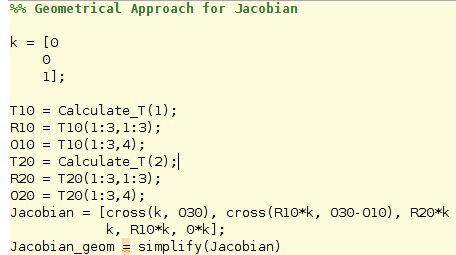
\includegraphics[width=0.5\textwidth]{Image6} % File
	\caption{Jacobian calculation by Geometrical Approach} % Name
	\label{fig:mesh6}
\end{figure}

And the result you can see in figure \ref{fig:mesh7}.

\begin{figure}[H]
	\centering
		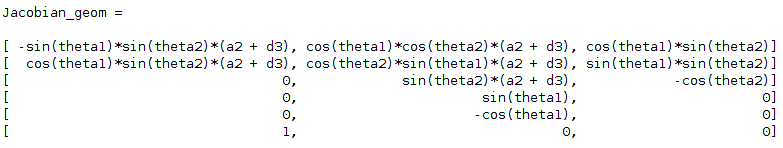
\includegraphics[width=1.0\textwidth]{Image7} % File
	\caption{Jacobian by Geometrical Approach} % Name
	\label{fig:mesh7}
\end{figure}

As you can see, it's the same as we got in classical approach, despite the difference that in this approach we have calculated $J_w$ part also.



\section*{Task 4:}
Analyze the Jacobian for singularities. Characterize each singular configuration if any.

{\centering
\subsection*{Solution}
}


There are a number of methods that can be used to determine the singularities of the Jacobian. Here, we will exploit the fact that a square matrix is singular when its determinant is equal to zero. But in general, it is difficult to solve the nonlinear equation det $J(q) = 0$.

The idea is that we partition the Jacobian J into 3 x 3 blocks as:

\begin{equation}
        J =
        \begin{bmatrix}
                J_{v}\\
               J_{w}\\
        \end{bmatrix}    
\end{equation}

And then find the dets of the parts to determine and analize the singularities.

So, I made the MATLAB code to determine the determinats. You can see it in the figure\ref{fig:mesh8}.

\begin{figure}[H]
	\centering
		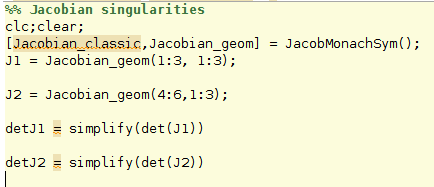
\includegraphics[width=0.5\textwidth]{Image8} % File
	\caption{Code to calculate Jacobian determinants} % Name
	\label{fig:mesh8}
\end{figure}


The result is the derminant which we must set equal to zero to determine singularities: 

\begin{equation}
        det{J\bm(q)_{v}} = sin(\theta_2+\frac{\pi}{2})(a_2+d_3)^2
\end{equation}

As we can see, determinant is equal to zero only when:
\begin{itemize}
	\item $d_3 = -a_2$. In our configuration, I think, it's impossible,because of no offsets.
	\item $\theta_2 = {\pi}k-\frac{\pi}{2}, k = \overline{1,n}$. It's the place, when our manipulator looks up or down. Like in the figure \ref{fig:mesh9}. Here are singularities because this positions have infinity amount of solutions.
\end{itemize}

\begin{figure}[H]
	\centering
	\begin{subfigure}[t]{0.5\textwidth}
		\centering
		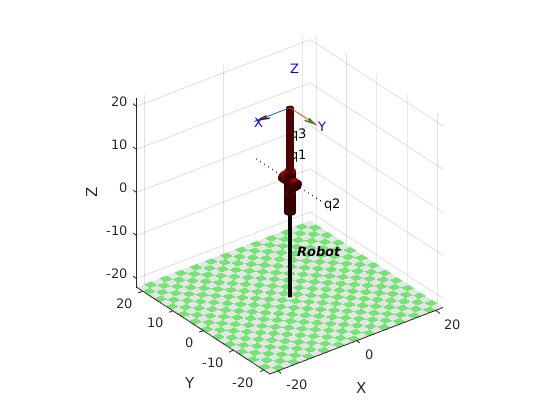
\includegraphics[width=0.7\textwidth]{Image9_1} % File
	\caption{"Up" Configuration} % Name
	\end{subfigure}%
	\begin{subfigure}[t]{0.5\textwidth}
		\centering
		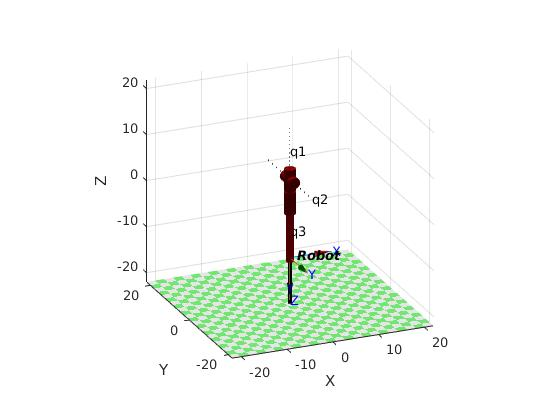
\includegraphics[width=0.7\textwidth]{Image9_2} % File
	\caption{"Down" Configuration} % Name
	\end{subfigure}%
	\caption{Singularities of the robot}
	\label{fig:mesh9}
\end{figure}


\section*{Task 5:}
Compute the velocity of the tool frame when joint variables are changing with time as follows:

{\centering
$\theta_1(t) = sin(t)$, $\theta_2(t) = cos(2t)$, $d_3(t) = sin(3t)$.
}

Add some fancy graphs showing evolution of all variables


{\centering
\subsection*{Solution}
}

For now, I have Jacobian of the robot in the symbolic view. Hence, I can substitute into the Jacobian Laws for $\theta_1$, $\theta_2$ and $d_3$ and then use the formula \ref{eq:18} to obtain tool frame velocities.

I also made MATLAB code, which algorithm is:
\begin{enumerate}
	\item Input movement laws for the joint variables.
	\item Calculate differentials of the joint variables.
	\item Substitute into the Jacobian Laws for $\theta_1$, $\theta_2$ and $d_3$.
	\item Calculate the tool frame velocities using formula \ref{eq:18}.
	\item Plot the result.	
\end{enumerate}

The fancy graphs you can see in the figure \ref{fig:mesh10}.

\begin{figure}[H]
	\centering
		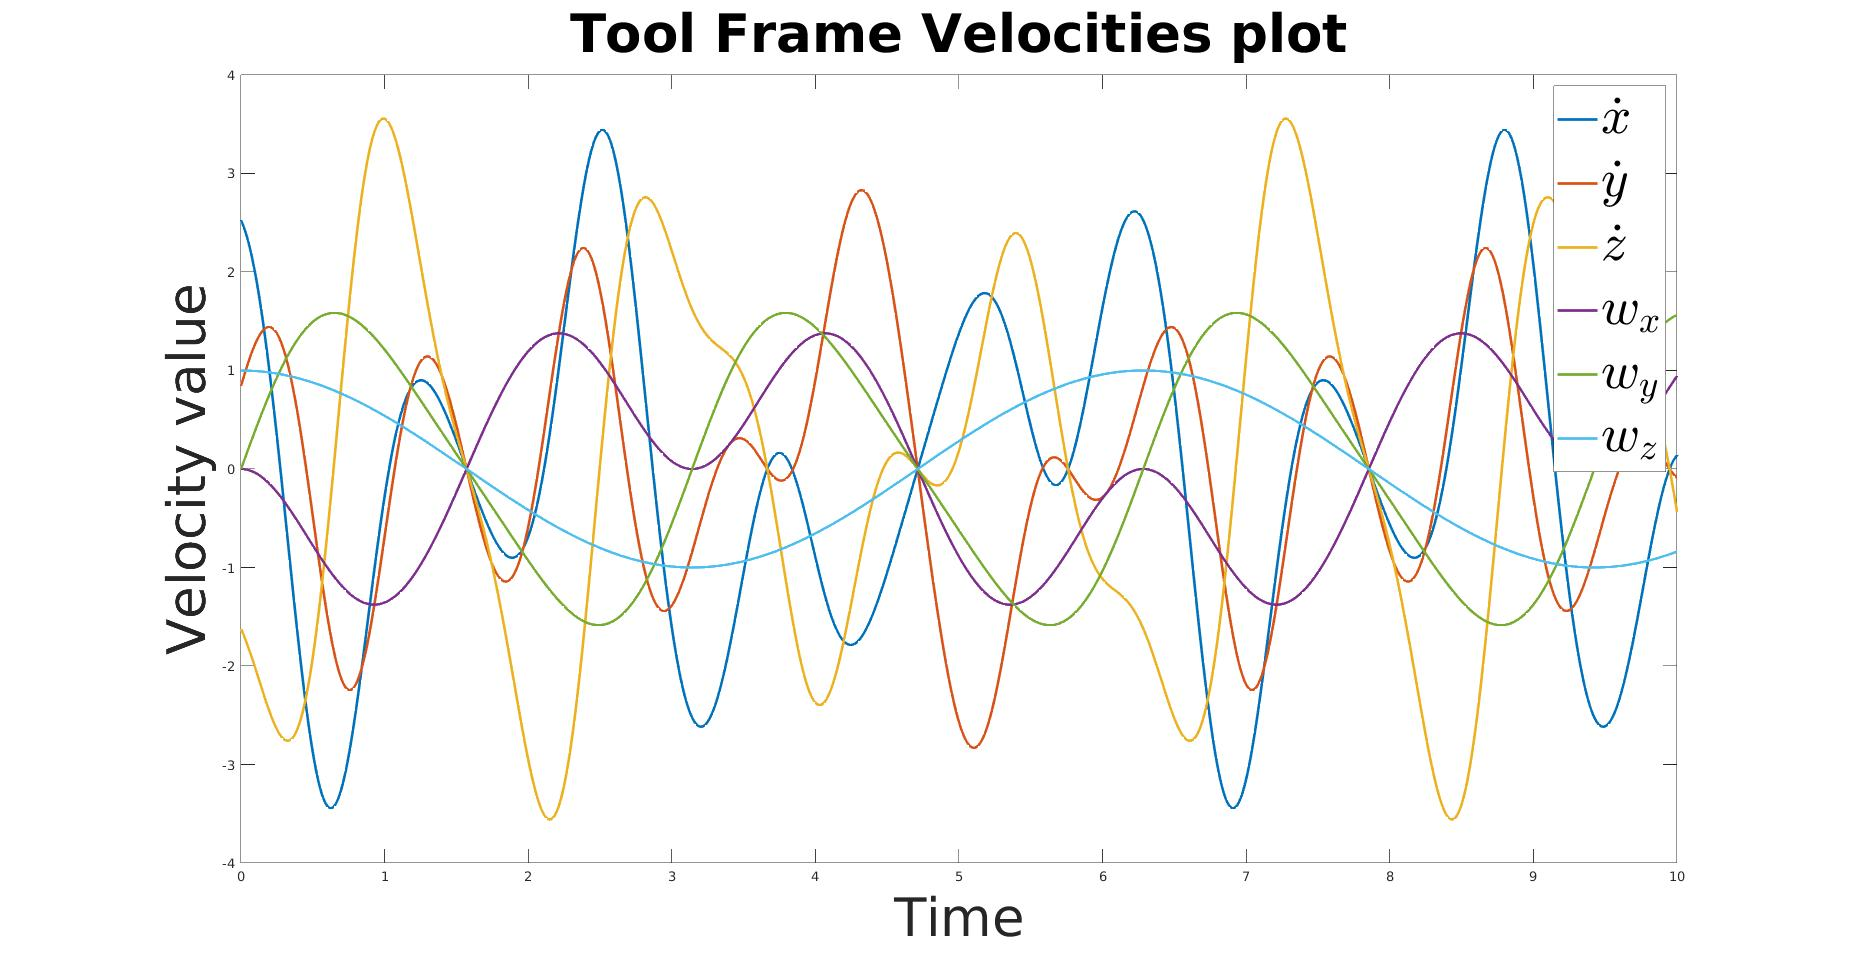
\includegraphics[width=1.0\textwidth]{Image10} % File
	\caption{Tool Frame Velocities plot} % Name
	\label{fig:mesh10}
\end{figure}

Formulas for Tool Frame Velocities you can see below:

{
\centering 
\begin{equation}
\fontsize{5}{12}\selectfont
        \begin{bmatrix}
                \dot{x}\\
                \dot{y}\\
                \dot{y} \\
                {w_x} \\
                {w_y} \\
                {w_z} \\
        \end{bmatrix}= 
\left(\begin{array}{c} 3\,\cos\left(3\,t\right)\,\cos\left(\sin\left(t\right)\right)\,\sin\left(\cos\left(2\,t\right)\right)-2\,\sin\left(2\,t\right)\,\cos\left(\sin\left(t\right)\right)\,\cos\left(\cos\left(2\,t\right)\right)\,\left(\sin\left(3\,t\right)+1\right)-\sin\left(\sin\left(t\right)\right)\,\sin\left(\cos\left(2\,t\right)\right)\,\cos\left(t\right)\,\left(\sin\left(3\,t\right)+1\right)\\ 3\,\cos\left(3\,t\right)\,\sin\left(\sin\left(t\right)\right)\,\sin\left(\cos\left(2\,t\right)\right)-2\,\sin\left(2\,t\right)\,\sin\left(\sin\left(t\right)\right)\,\cos\left(\cos\left(2\,t\right)\right)\,\left(\sin\left(3\,t\right)+1\right)+\cos\left(\sin\left(t\right)\right)\,\sin\left(\cos\left(2\,t\right)\right)\,\cos\left(t\right)\,\left(\sin\left(3\,t\right)+1\right)\\ -3\,\cos\left(3\,t\right)\,\cos\left(\cos\left(2\,t\right)\right)-2\,\sin\left(2\,t\right)\,\sin\left(\cos\left(2\,t\right)\right)\,\left(\sin\left(3\,t\right)+1\right)\\ -2\,\sin\left(2\,t\right)\,\sin\left(\sin\left(t\right)\right)\\ 2\,\sin\left(2\,t\right)\,\cos\left(\sin\left(t\right)\right)\\ \cos\left(t\right) \end{array}\right)
\fontsize{12}{12}\selectfont
\end{equation}
}

\section*{Task 6:}
Let tool coordinates changing with time as follows:

{\centering
$p_x(t) = 2a_2sin(t)$, $p_y(t) = 2a_2cos(2t)$, $p_z(t) = d_1sin(3t)$
}

Determine a feasible joint trajectory for this tool trajectory.

\begin{itemize}
	\item Use IK solution.
	\item Use inverse differential kinematics approach. Consider only linear
velocity part of Jacobian.
\end{itemize}

{\centering
\subsection*{Solution}
}


{\centering
\subsubsection*{Using IK solution for joint trajectories}
}

We know the tool coordinates changing. Also, I have solved the IK problem before in the section \nameref{sec:Task 2}.

Hence, I made MATLAB code for IK solving and put tool coordinates changing in it to obtain joints' movements.

The results you can see below in figures \ref{fig:mesh11}-\ref{fig:mesh12}.

\begin{figure}[H]
	\centering
		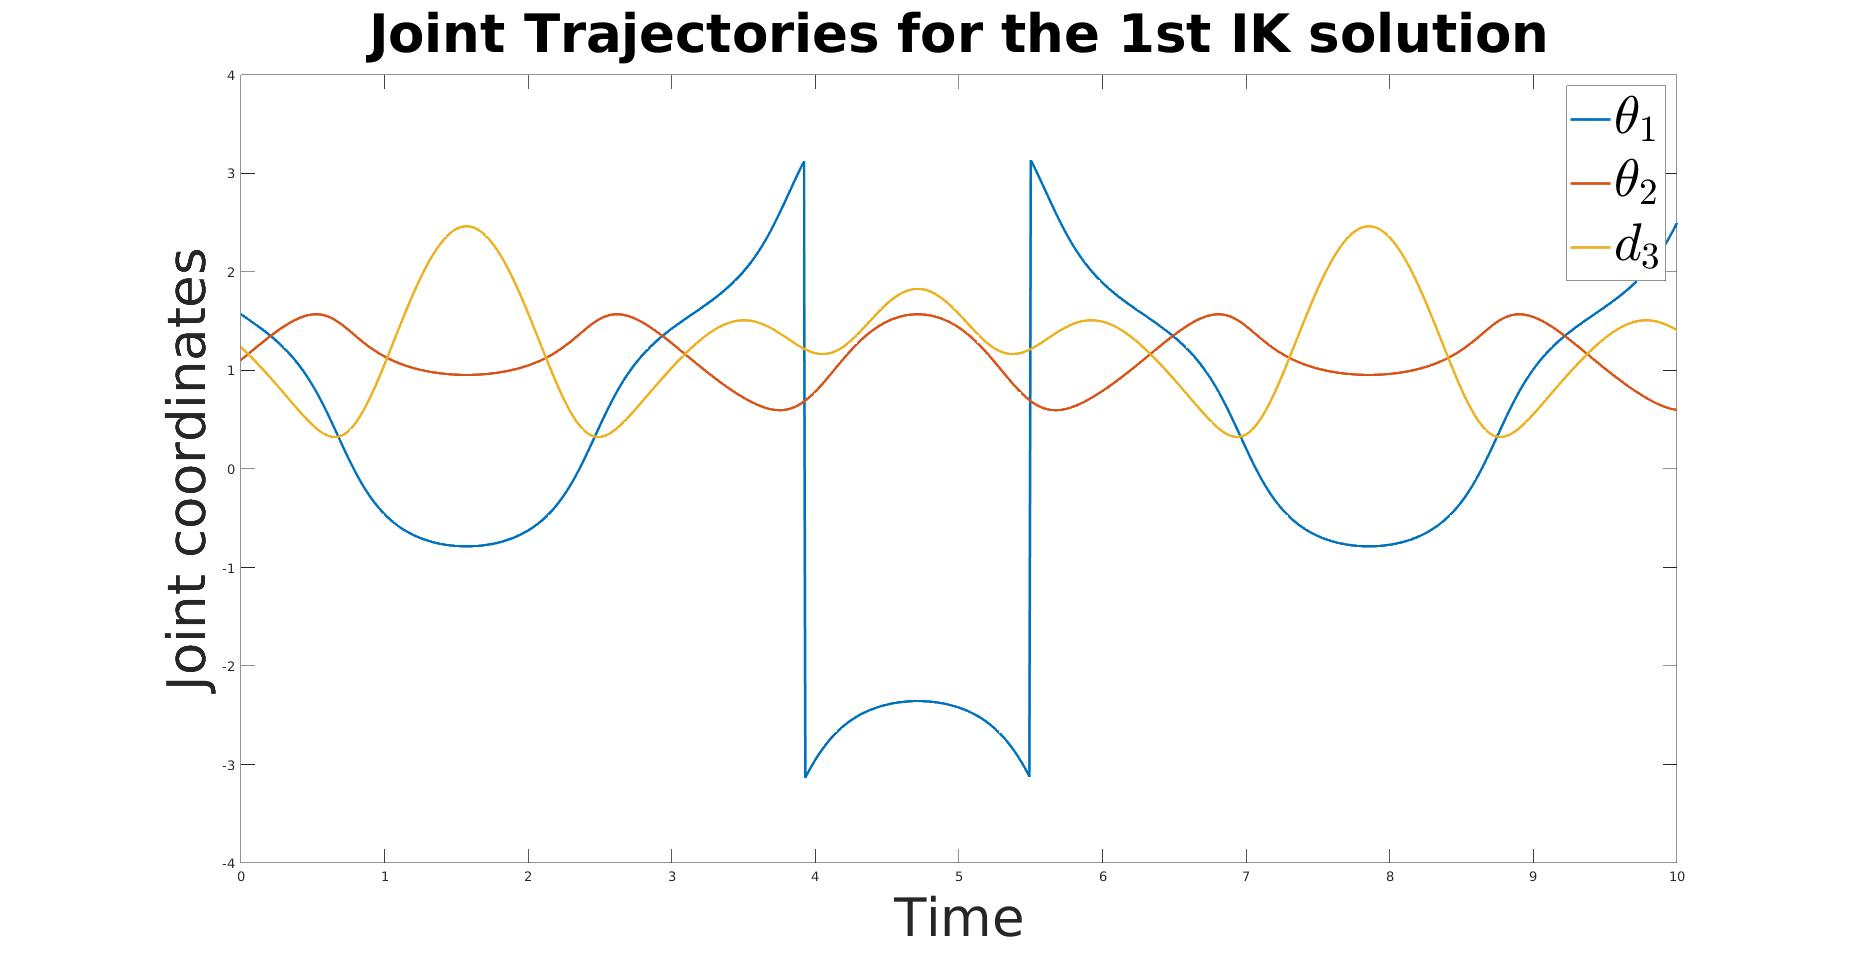
\includegraphics[width=1.0\textwidth]{Image11} % File
	\caption{Joint Trajectories for the 1st IK solution} % Name
	\label{fig:mesh11}
\end{figure}

\begin{figure}[H]
	\centering
		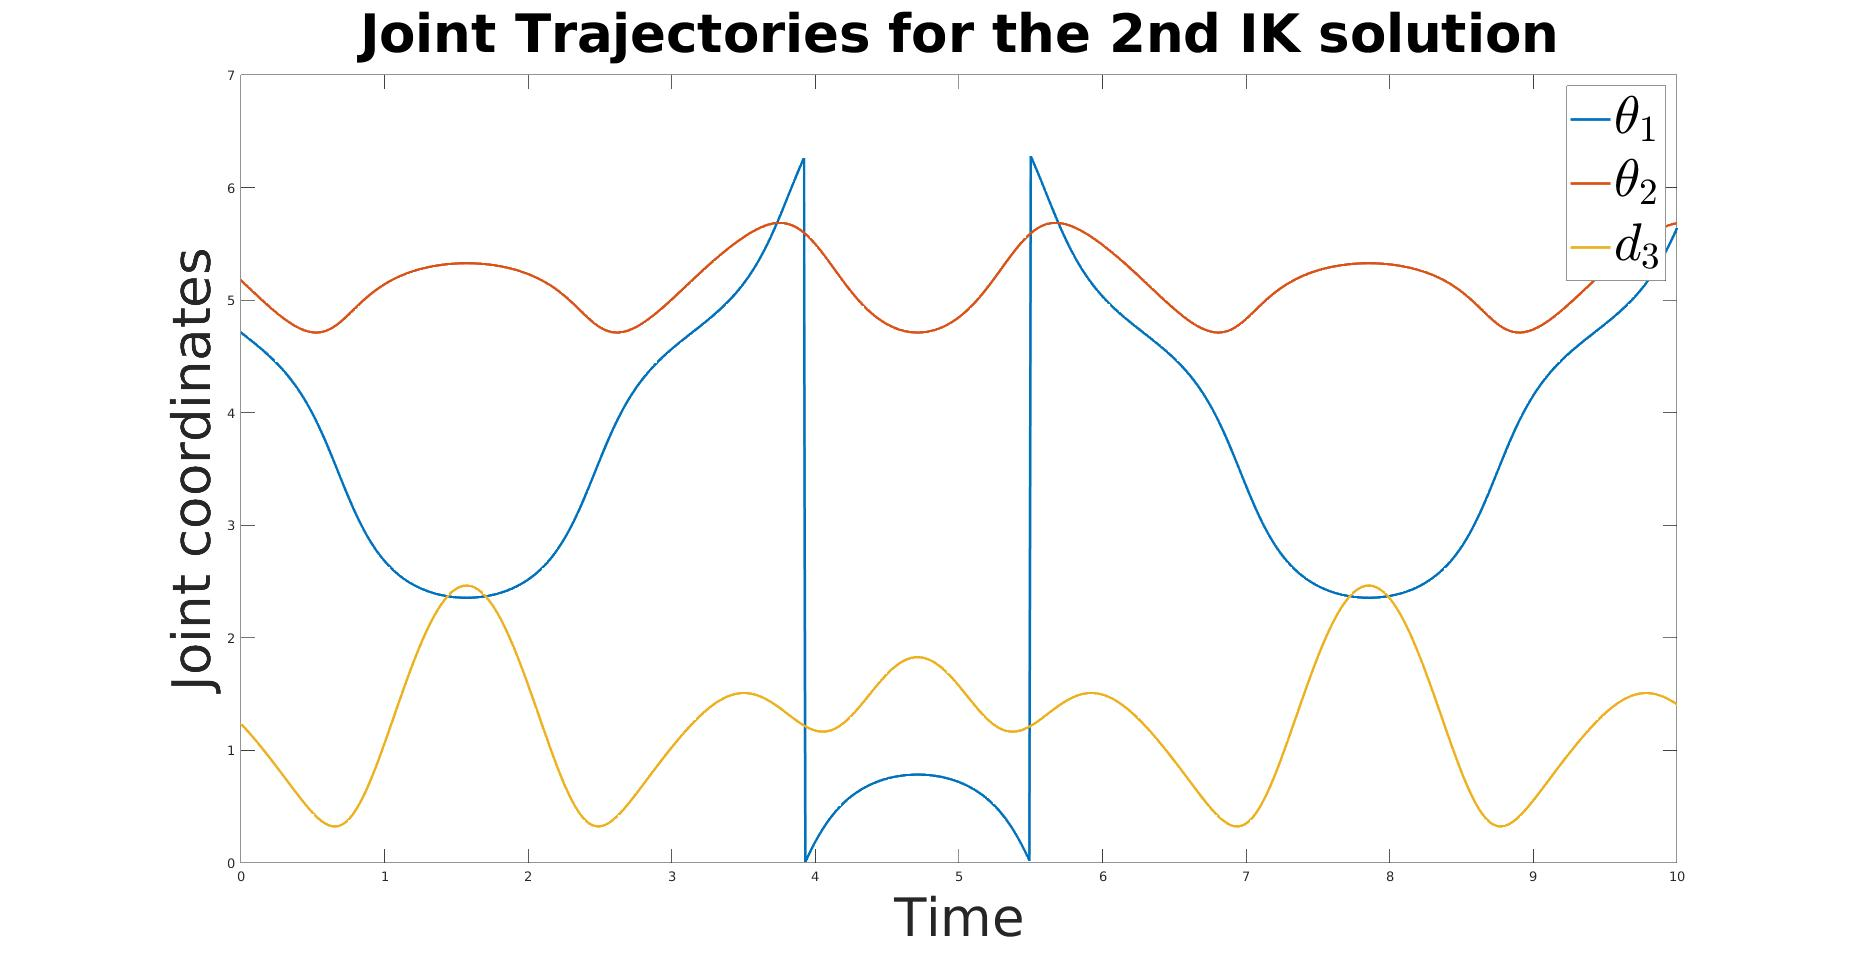
\includegraphics[width=1.0\textwidth]{Image12} % File
	\caption{Joint Trajectories for the 2nd IK solution} % Name
	\label{fig:mesh12}
\end{figure}

The video of plotting the robot and it's desired (red) and actual (blue) paths (part of it) you can find \href{https://drive.google.com/open?id=1xH5_-XHiQtQv5W_jp0Rq1UXxTakYNbU7}{here}.

The whole code for HA you can find \href{https://github.com/Terminateit/HA3Dynamics-.git}{here}.

{\centering
\subsubsection*{Using inverse differential kinematics approach for joint trajectories}
}

The idea is that we have \ref{eq:18} and we want to calculate $\dot{\bm{q}}$:

\begin{equation}
        \dot{\bm{q}} = J^{-1}\begin{bmatrix}
                \dot{x}\\
                \dot{y}\\
                \dot{y} \\
                {w_x} \\
                {w_y} \\
                {w_z} \\
        \end{bmatrix}
\end{equation}

After that, we solve the system of differential equations to obtain ${\bm{q}}$.

Also, as usual, I made MATLAB code to solve this problem and plot the results. 

The video of plotting the robot and it's desired (red) and actual (blue) paths (part of it) you can find \href{https://drive.google.com/open?id=1SzXLqlq0qzzBGzvQZjL8gK2-DVrcIFDe}{here}.

As I concluded, the both methods give pretty the same results and the error is quite miserable.
\end{document}